\chapter{Background}

This thesis is meant for the general computer science public, and so we will provide some background on the tools and technologies used in this thesis. We will also provide some background on capitalization tables and ecossystem of software solutions, including the OpenCapTable Format.

\section{Overview of Alloy and JSON Schema}

We use two languages in this thesis: Alloy and JSON Schema.

Alloy is a language for describing models in first-order logic and the Alloy Analyzer is a tool for analyzing such models. JSON Schema is a data validation format for JSON documents, with a JSON-based syntax.

\subsection{Overview of Alloy}

Alloy\cite{DJSALLA} is a formal specification language and analysis tool developed by Daniel Jackson and his colleagues at the Massachusetts Institute of Technology (MIT). Alloy allows users to define abstract models of complex systems and to automatically check their properties using a bounded model checking algorithm. Alloy's syntax is based on first-order logic and set theory, and includes constructs for defining relations, functions, and constraints.

\noindent An Alloy model consists of the following parts:

\begin{itemize}
	\item Signature declarations, labeled by a \verb|sig| keyword, introduce a set of \textit{atoms} and a set of \textit{fields} relating atoms. A signature is similar but more general than a SQL table, for example.
	\item Constraint declarations, introduced by the keywords \verb|fact|, \verb|fun|, and \verb|predicate|, that limit the possible instances of the model. Facts are assumed to always hold.  Functions are reusable, named expressions, that return a relation. Predicates are functions that must evaluate to a boolean.
	\item Assertion declarations, introduced by the keyword \verb|assert|, that establish constraints that are expected to hold as consequences of the facts. Assertions can be checked by the Alloy Analyzer using the \verb|check| command.
\end{itemize}

Using the \verb|run| and \verb|check| commands, the user can ask the Alloy Analyzer to find examples and counter examples to expressions (usually built up from predicates) in a given \textit{scope}. The scope determines how many atoms can be created in the model (by signature). A larger scope is populated by more instances, but takes longer to check.

\subsubsection{Advantages of Alloy}

One of the key benefits of Alloy is its ability to quickly generate and evaluate different scenarios and configurations, allowing designers to iteratively refine their models and identify potential issues.

Alloys' value proposition is to take the ideal of precise and expressive notation based on a tiny core of simple and robust concepts, but it replace basic analysis based on theorem proving with a fully automatic analysis with immediate feedback.\cite{DJSALLA}

\begin{figure}
\centering
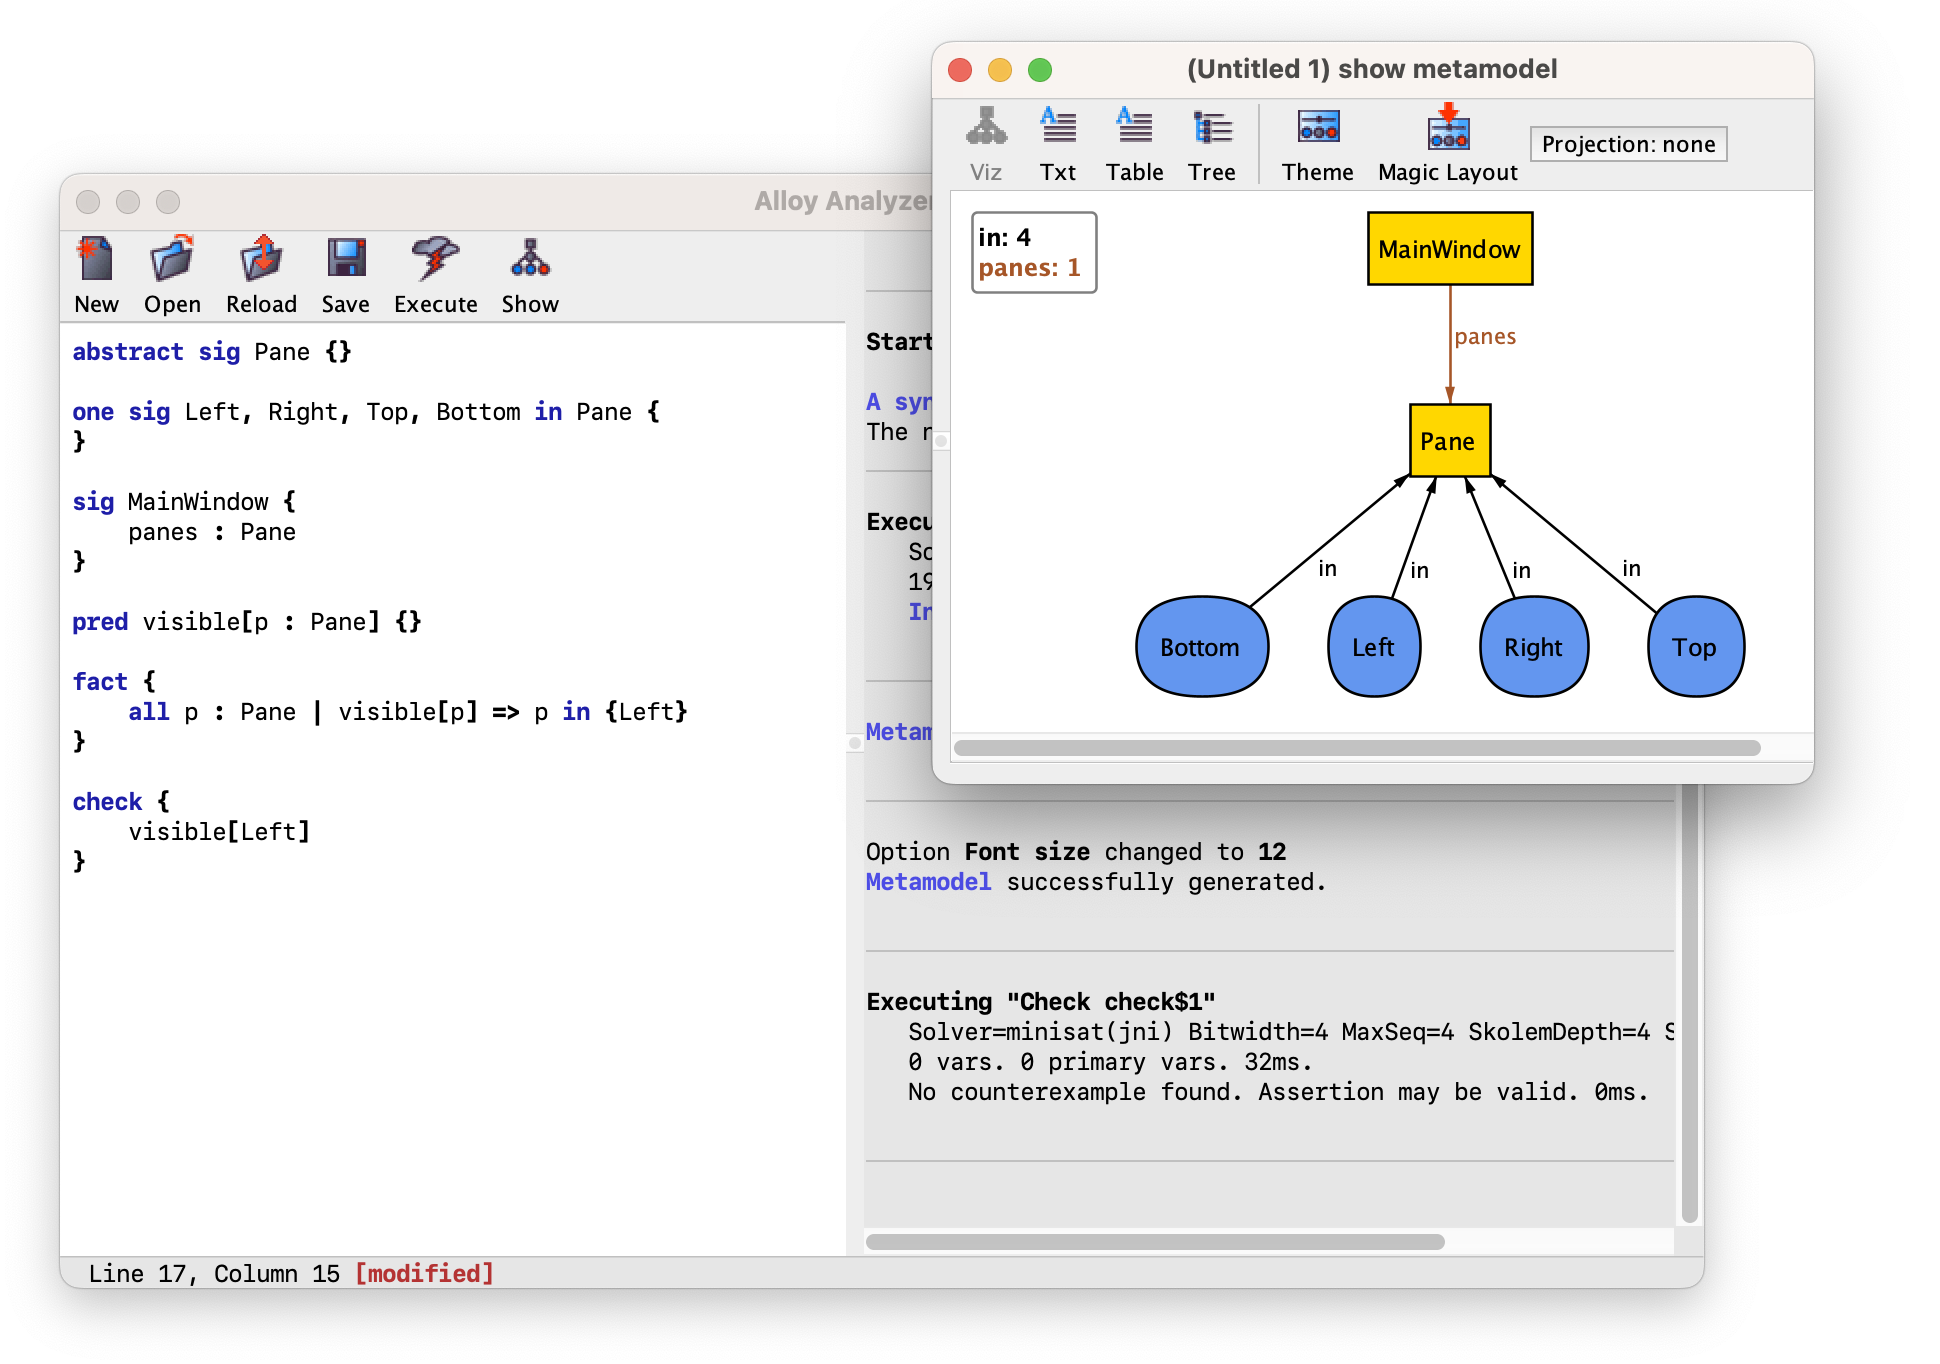
\includegraphics[width=0.8\textwidth]{pics/alloy-analyzer.png}
\caption{Alloy Analyzer}\label{fig:alloy-analyzer}
\end{figure}

\subsubsection{Applications of Alloy}

Alloy has been used in a wide range of applications in computer science, including software engineering, database design, security analysis\cite{Carpio2021}\cite{Chen2006}, multi-agent negotiations \cite{Podorozhny}. It has also been applied to modeling beyond computer science such as a model for central bank policy\cite{Johnson2021}. A model of the same-origin-policy used in web browsers can be found in the 500 Lines or Less open-source book\cite{500Lines19:online}. Alloy$\ast$ is a higher-order extension of Alloy that can be used for program synthesis, since it supports higher-order quantification\cite{Milicevic2017}. $\alpha{Rb}y$ is an embedding of Alloy in Ruby\cite{Arby}.


\subsection{Overview of JSON Schema}

JSON Schema, a specification for JSON (JavaScript Object Notation) data, provides a systematic approach to define the structure and constraints of JSON data. JSON, a lightweight data interchange format, is ubiquitously employed in web applications and APIs due to its simplicity and readability. JSON Schema, utilizing a JSON-based syntax, allows developers to meticulously define the structure and constraints of JSON data. A comprehensive description of JSON Schema is provided in RFC8259\cite{RFC8259}.

The versatility of JSON Schema is evident in its extensive range of validation rules and constraints. These include, but are not limited to, data types, required fields, minimum and maximum values, and regular expressions. Furthermore, JSON Schema supports custom validation rules and extensions, thereby offering developers the flexibility to define their own rules and constraints. This feature significantly enhances the adaptability of JSON Schema to cater to diverse and specific requirements.

JSON Schema is a powerful tool that leverages the simplicity and readability of JSON, making it human-friendly and easy to comprehend. It employs hypermedia principles, allowing schemas to reference other schemas through a Universal Resource Identifier (URI). This feature enhances the modularity and reusability of schemas, thereby promoting efficient schema design and management.

In the context of designing messages for HTTP application programming interfaces (APIs), JSON Schema proves to be exceptionally adequate. It provides robust validation capabilities, ensuring the integrity and consistency of data communicated through APIs. Not only can it validate the presence of all necessary arguments, but it also offers basic format validation. This means it can check if the data conforms to the specified types, patterns, or other constraints, thereby ensuring that the data received or sent via APIs adheres to the expected structure and format. This comprehensive validation capability significantly enhances the reliability and robustness of HTTP APIs, making JSON Schema an indispensable tool in modern web development.

See table \ref{tab:json-schema-validation-keywords} for a list of validation keywords.

\begin{table}[h!]
\centering
	\begin{tabular}{|l|p{10cm}|}
		\hline
		\textbf{Validation Keyword} & \textbf{Description}                                                          \\
		\hline
		type                        & Specifies the data type (e.g., string, number, object, array, boolean, null)  \\
		\hline
		enum                        & Specifies a predefined list of acceptable values                              \\
		\hline
		const                       & Specifies a constant value that the data must match                           \\
		\hline
		multipleOf                  & Specifies that a numeric instance is divisible by this keyword's value        \\
		\hline
		maximum                     & Specifies the maximum numeric value                                           \\
		\hline
		exclusiveMaximum            & Specifies a numeric instance to be strictly less than this keyword's value    \\
		\hline
		minimum                     & Specifies the minimum numeric value                                           \\
		\hline
		exclusiveMinimum            & Specifies a numeric instance to be strictly greater than this keyword's value \\
		\hline
		maxLength                   & Specifies the maximum length of a string                                      \\
		\hline
		minLength                   & Specifies the minimum length of a string                                      \\
		\hline
		pattern                     & Specifies a regular expression that a string must match                       \\
		\hline
		items                       & Specifies constraints for array items                                         \\
		\hline
		maxItems                    & Specifies the maximum number of items in an array                             \\
		\hline
		minItems                    & Specifies the minimum number of items in an array                             \\
		\hline
		uniqueItems                 & Specifies that all items in an array must be unique                           \\
		\hline
		properties                  & Specifies constraints for object properties                                   \\
		\hline
		required                    & Specifies required properties in an object                                    \\
		\hline
		additionalProperties        & Specifies whether additional properties are allowed                           \\
		\hline
	\end{tabular}
\caption{Available Validations in JSON Schema}
\label{tab:json-schema-validation-keywords}
\end{table}
  
\subsubsection{Tooling for JSON Schema}

JSON Schema is supported by a large number of tools\cite{jsonschemaImplementations}: validators, schema generators and code generators. There are validators for all major languages, and the schema generators can generate schemas from code, data and models. Code generators can implement basic Web-based user interfaces and generate data based on schemas.

There is also a noteworthy repository of JSON Schemas for hundreds of APIs, called JSON Schema Store\cite{schemastoreJSONSchema}.

\subsection{Mapping from JSON Schema to Alloy}

Here we describe our general approach for translating JSON Schema into Alloy. Basically, we follow the steps:

\begin{figure}[ht!]
\centering
	\begin{minipage}{.8\linewidth}
		\begin{enumerate}
			\item\label{itm:abstract_signature} Translate the \textit{schemas} into \textit{abstract signatures} in Alloy, devoid of any fields.
			\item\label{itm:concrete_signature} Iterate over each \textit{abstract signature} from step \ref{itm:abstract_signature}. For each, instantiate it into a \textit{concrete signature} and incorporate the corresponding fields as specified in the JSON schema.
			\item\label{itm:related_signatures} Examine each field from step \ref{itm:concrete_signature}. Consequently, introduce the pertinent signatures into our \textit{stack} and return to step \ref{itm:concrete_signature}.
			\item\label{itm:assertions} Formulate \textit{assertions} which are anticipated to be upheld given the domain currently being modeled.
			\item\label{itm:analyzer} Employ the \textit{Alloy Analyzer} to assess whether the assertions from step \ref{itm:assertions} are satisfied. If not, progress to the subsequent step.
			\item\label{itm:constraint} Extend the Alloy model with a fresh \textit{constraint} if the assertions from step \ref{itm:assertions} were not satisfied. Repeat steps from \ref{itm:concrete_signature} to \ref{itm:constraint} until all assertions hold true.
		\end{enumerate}
	\end{minipage}
\caption{Process of creating an Alloy model from schemas}
\label{fig:json-to-alloy-translation-algorithm}
\end{figure}  

Our scheme implements a depth-first search of the original schema, and when completed, the Alloy model should be a roughly direct translation of the original schema. Once this is done, we can start improving the model using the more expressive semantics of Alloy, always checking if the assertions hold.

\section{What are Capitalization Tables?}

Formally, a capitalization table can be defined as a mapping of the set of stakeholders in a company to the number of shares they own in each asset class in the company. In this thesis we consider common stocks and stock options as asset classes. Mathematicall, assuming $S$ is the set of stakeholders, $A$ is the set of asset classes, a capitalization table at date $t$ is a function $C_t: S \times A \rightarrow \mathbb{N}$.

\subsection{Overview of Capitalization Tables}


A capitalization table is a snapshot of the relationship of stakeholders in a company and the number of shares they own in each asset class in the company. In this thesis we consider common stocks and stock options as asset classes.

\begin{table}[h!]
\centering
	\begin{tabular}{|l|l|l|l|l|}
		\hline
		Investor       & Asset Class     & Shares & Cost (USD) & \% of Company \\
		\hline
		Founders       & Common Stock    & 10,000 & -          & 71.43\%       \\
		Seed Investors & Preferred Stock & 2,000  & 2,000,000  & 14.29\%       \\
		Option Pool    & Common Stock    & 2,000  & -          & 14.29\%       \\
		\hline
		Total          & -               & 14,000 & 2,000,000  & 100.00\%      \\
		\hline
	\end{tabular}
\caption{Example of a capitalization table}
\label{tab:example-capitalization-table}
\end{table}

Here, the set of stakeholders $S$ is $\{ \text{Founders}, \text{Seed Investors}, \text{Option Pool} \}$, and the set of asset classes $A$ is $\{ \text{Common Stock}, \text{Preferred Stock} \}$. The capitalization table is a function $C: S \times A \rightarrow \mathbb{N}$, where $C(\text{Founders}, \text{Common Stock}) = 10,000$, $C(\text{Seed Investors}, \text{Preferred Stock}) = 2,000$, and so on.

Changes in a capitalization table are effects from transactions (both in the business sense, but also in the computing sense): issuance of shares to new investors, transfers of shares between investors, and formation of pools for and exercise of stock options by employees.

\begin{tikzpicture}[
    >=stealth,
    node distance=2cm,
    pil/.style={
        ->,
        thick,
        shorten <=2pt,
        shorten >=2pt,}
]
  
\node[rectangle,draw] (empty) {EmptyCapTable};
\node[rectangle,draw,right=of empty] (cap1) {CapTable1};
\node[rectangle,draw,right=of cap1] (cap2) {CapTable2};
\node[rectangle,draw,right=of cap2] (cap3) {CapTable3};
  
\path[pil] (empty) edge [above] node [yshift=12pt] {Company constitution} (cap1);
\path[pil] (cap1) edge [above] node [yshift=12pt] {Seed round} (cap2);
\path[pil] (cap2) edge [above] node [yshift=12pt] {Series A round} (cap3);
  
\end{tikzpicture}

\subsubsection{Why are Capitalization Tables Important?}

Cap tables are important for several reasons. First, they provide a clear and accurate picture of the ownership structure of the company, which is crucial for decision-making and financial reporting. Second, they help to ensure that equity is distributed fairly and transparently among shareholders. Finally, they can be used to calculate the potential payouts and returns for different scenarios, such as a sale of the company or an initial public offering (IPO). A venture capital firm may use a cap table to track the ownership and value of its portfolio companies. The cap table can help the firm to make informed decisions about future investments, and can help to identify potential exit opportunities.


Critically, the cap table can help to ensure that the ownership and value of the company is distributed fairly among investors and founders, and can help to identify potential issues or conflicts.

\subsubsection{How are Capitalization Tables Used?}

Here are the typical operations in startup financing. All have effects on the final capitalization table.

\begin{longtable}[h!]{|p{5cm} | p{8cm}|} 
\caption{Common startup financing operations} \\
	\hline
	\textbf{Operation}         & \textbf{Description}                                                                                           \\ [0.5ex] 
	\hline
	\endfirsthead
	
	\multicolumn{2}{c}%
	{\tablename\ \thetable\ -- \textit{Continued from previous page}} \\
	\hline
	\textbf{Operation}         & \textbf{Description}                                                                                           \\ [0.5ex]
	\hline\hline
	\endhead
	
	\hline \multicolumn{2}{r}{\textit{Continued on next page}} \\
	\endfoot
	
	\hline
	\endlastfoot
	
	Equity financing           & Money from investors is converted into shares at a given price-per-share                                       \\ 
	Convertible note financing & Money from investors is lent to the company as debt, but with a provision to convert into shares in the future \\ [1ex]
	Employee stock options     & Employees are given the right to purchase shares at a given price-per-share in the future                      \\ [1ex]
	\hline
\end{longtable}
\subsection{Examples}

\textbf{Seed round with convertible debt}

\vskip1cm

Here a new startup has only founders in its capitalization table. The founders have 10,000 shares. The company raises \$1,0M in a convertible note financing. The convertible note has a \$20M valuation cap. The convertible note converts into shares at the next equity financing round. Thus, shares can be given as actually issued shares and fully diluted shares, which are estimates based on corresponding schedule stock issuances.

\vskip1cm

\begin{center}
	\begin{tabular}{|p{3cm}|p{3cm}|p{3cm}|}
		\hline
		Shareholder  & Shares & Percentage \\
		\hline
		Founders     & 10,000 & 100\%      \\
		\hline
		Total        & 10,000 & 100\%      \\
		\hline
		Common Stock & 10,000 & 100\%      \\
		\hline
	\end{tabular}
	
\end{center}

\vskip1cm

\begin{center}
	\begin{tabular}{|p{3cm}|p{3cm}|p{3cm}|p{3cm}|}
		\hline
		Shareholder       & Shares   & Shares          & Percentage \\
		                  & (Actual) & (Fully Diluted) &            \\
		\hline
		Founders          & 10,000   & 10,000          & 95\%       \\
		\hline
		Investor I (Debt) & 0        & 526.32          & 5\%        \\
		\hline
		Total             & 10,000   & 10,526.32       & 100\%      \\
		\hline
	\end{tabular}
\end{center}

\subsubsection{Problems in managing capitalization tables}

Cap tables may change frequently, reflecting changes in ownership, investment, and valuation over time. They are complex to manage and validate, because they are only a snapshot, a state. A cap table can only be verified in trivial ways \- sums and percentages not adding up. 

But the financial operations and transactions that evolve a capitalization table must comply with a series of legal and business rules that are ultimately defined in business contracts, and software to do so must take into account the following:

\begin{enumerate}
	\item Avoid double spending and ensuring the overall life of a security is correct (it must be created once and spent only if ever created, and it can undergo non-terminal transactions)
	\item No cycles should be possible in the life cycle of any security (a security can not be both the input and output of a single transaction or a set of transactions such as a partial cancellation that creates a residual security)
	\item Support very complex business rules that are defined in business contracts, and that are not trivial even to specify
	\item Respect basic accounting equations such as that the number of shares in circulation must never exceed the number of shares created
\end{enumerate}

Which are reflected in our research questions.

\section{Ecossystem and The Open Cap Table Format}

In the last decade (2010-2020), a number of software-as-a-service solutions have emerged in the capitalization table management and related spaces in various geographies. These solutions are not interoperable, and there is no standard for exchanging capitalization table data.

The Open Cap Table Format (OCF) is a data interchange format for capitalization tables. It is a JSON Schema-based format that is designed to be easy to use and understand. The OCF is intended to be used by startups, investors, and other stakeholders in the venture capital market.

In the next chapter, we will give a detailed description of the OCF, and in the following chapters we will provide a translation of the most important parts of the OCF into an Alloy specification.

% Solutions in the space
% Carta, founded as eShares in 2012, specializes in capitalization table management, with reportedly 2.4M users and USD 2.5tn in assets in the platform.
% Shareworks, founded in 1999 and now owned by Morgan Stanley, manages capitalization tables and also offers compensation financial planning solutions for employees\cite{Sharewor68:online}.
% The Long-term Stock Exchange, is stock exchange founded in 2015 focused on long-term value creation, has a cap table management solution\cite{LTSEHome63:online} with reportedly 40,000 startup founders using it.
% Create a nice table: company, founded at and description
\begin{tabular}{|l|l|p{6cm}|}
\hline
\textbf{Company}                                 & \textbf{Founded} & \textbf{Geography} \\ \hline
Shareworks\cite{Sharewor68:online}               & 1999             & USA                \\ \hline
Carta\cite{CartaEqu70:online}                    & 2012             & USA                \\ \hline
Long-term Stock Exchange\cite{LTSEHome63:online} & 2015             & USA                \\ \hline
Raise\cite{Software0:online}                     & 2018             & Africa             \\ \hline
Distu\cite{DistuEqu4:online}                     & 2021             & Brazil             \\ \hline
\end{tabular}

